%Made By Thomas Debelle
%Ajouté des Packages si nécessaires
\documentclass{report}
\usepackage[a4paper, total={6in, 9in}]{geometry}
\usepackage[utf8]{inputenc}
\usepackage[english]{babel}
\usepackage{graphicx}
\usepackage{graphics}
\usepackage[T1]{fontenc}
\usepackage{amsmath}
\usepackage{hyperref}
\usepackage{amssymb}
\usepackage{booktabs}
\usepackage{listings}
\usepackage{xcolor}
\usepackage{array}
\usepackage{float}
\usepackage{amsfonts}
\usepackage{fancyhdr}
\usepackage{titlesec}
\usepackage{xparse}
\usepackage{wrapfig}
\usepackage{glossaries}

\makeglossaries


\hypersetup{
    colorlinks=true,
    linkcolor=black,
    filecolor=magenta,
    urlcolor=cyan,
    pdftitle={Overleaf Example},
    pdfpagemode=FullScreen,
    }
\begin{document}
\newacronym{mfp}{MFP}{Mean Free Path}
\newglossaryentry{mfpdef}{
    type=definitions,
    name={Mean Free Path (MFP)},
    description={The average distance a particle (such as an electron, atom, or molecule) travels between collisions. In semiconductors and thin films, it influences transport phenomena.}
}

\newacronym{cvd}{CVD}{Chemical Vapor Deposition}
\newglossaryentry{cvddef}{
    type=definitions,
    name={Chemical Vapor Deposition (CVD)},
    description={A process where gaseous precursors chemically react or decompose on a substrate surface to form a solid material, often used for thin-film fabrication in semiconductor manufacturing.}
}


\newacronym{pvd}{PVD}{Physical Vapor Deposition}
\newglossaryentry{pvddef}{
    type=definitions,
    name={Physical Vapor Deposition (PVD)},
    description={A vacuum-based process in which material is physically vaporized and deposited onto a substrate to form thin films.}
}

\newacronym{mbe}{MBE}{Molecular Beam Epitaxy}
\newglossaryentry{mbedef}{
    type=definitions,
    name={Molecular Beam Epitaxy (MBE)},
    description={An ultra-high vacuum technique where atomic or molecular beams are directed at a heated substrate to grow highly controlled epitaxial layers.}
}

\newacronym{ald}{ALD}{Atomic Layer Deposition}
\newglossaryentry{alddef}{
    type=definitions,
    name={Atomic Layer Deposition (ALD)},
    description={A vapor-phase technique for depositing thin films one atomic layer at a time using sequential, self-limiting reactions. Offers excellent conformality.}
}

\newacronym{sti}{STI}{Shallow Trench Isolation}
\newglossaryentry{stidef}{
    type=definitions,
    name={Shallow Trench Isolation (STI)},
    description={A process used to isolate CMOS transistors on a silicon wafer by etching shallow trenches and filling them with dielectric material.}
}

\newacronym{dti}{DTI}{Deep Trench Isolation}
\newglossaryentry{dtidef}{
    type=definitions,
    name={Deep Trench Isolation (DTI)},
    description={An isolation method using deep etched trenches filled with insulators, used in 3D integration and high-voltage devices.}
}

\newacronym{locos}{LOCOS}{LOCal Oxidation of Silicon}
\newglossaryentry{locosdef}{
    type=definitions,
    name={LOCal Oxidation of Silicon (LOCOS)},
    description={A technique for selectively growing oxide on silicon for isolation by locally exposing regions to thermal oxidation.}
}

\newacronym{teos}{TEOS}{TEtraethylorthOSilicate}
\newglossaryentry{teosdef}{
    type=definitions,
    name={TEtraethylorthOSilicate (TEOS)},
    description={A silicon precursor used in CVD to deposit silicon dioxide films. TEOS provides good conformality and uniformity.}
}

\newacronym{cmp}{CMP}{Chemical-Mechanical Polishing}
\newglossaryentry{cmpdef}{
    type=definitions,
    name={Chemical-Mechanical Polishing (CMP)},
    description={A planarization process combining chemical slurry and mechanical abrasion to produce flat surfaces in semiconductor fabrication.}
}

\newacronym{lto}{LTO}{Low-temperature Oxidation}
\newglossaryentry{ltodef}{
    type=definitions,
    name={Low-temperature Oxidation (LTO)},
    description={A thermal oxidation process performed at lower temperatures to form silicon dioxide, used when high-temperature processing is not feasible.}
}

\newacronym{hto}{HTO}{High-temperature Oxidation}
\newglossaryentry{htodef}{
    type=definitions,
    name={High-temperature Oxidation (HTO)},
    description={An oxidation process performed at high temperatures to produce high-quality oxide films on silicon.}
}

\newacronym{pecvd}{PECVD}{Plasma Enhanced CVD}
\newglossaryentry{pecvddef}{
    type=definitions,
    name={Plasma Enhanced CVD (PECVD)},
    description={A variant of CVD where plasma is used to enhance chemical reactions, enabling deposition at lower temperatures.}
}

\newacronym{lpcvd}{LPCVD}{Low Pressure CVD}
\newglossaryentry{lpcvddef}{
    type=definitions,
    name={Low Pressure CVD (LPCVD)},
    description={A CVD process carried out under reduced pressure, leading to better uniformity and fewer contaminants.}
}

\newacronym{arc}{ARC}{Anti Reflective Coating}
\newglossaryentry{arcdef}{
    type=definitions,
    name={Anti Reflective Coating (ARC)},
    description={A thin film applied to reduce reflections and improve pattern fidelity in photolithography.}
}

\newacronym{rta}{RTA}{Rapid Thermal Annealing}
\newglossaryentry{rtadef}{
    type=definitions,
    name={Rapid Thermal Annealing (RTA)},
    description={A process of quickly heating wafers to activate dopants or repair damage without significantly affecting the rest of the structure.}
}

\newacronym{sims}{SIMS}{Secondary Ion eMission Spectroscopy}
\newglossaryentry{simsdef}{
    type=definitions,
    name={Secondary Ion eMission Spectroscopy (SIMS)},
    description={An analytical technique that sputters a sample surface and detects secondary ions to determine composition and depth profiles.}
}

\newacronym{srp}{SRP}{Spreading Resistance Profilometry}
\newglossaryentry{srpdef}{
    type=definitions,
    name={Spreading Resistance Profilometry (SRP)},
    description={A technique for measuring the resistivity and doping profile of semiconductors by placing probes along a beveled surface.}
}

\newacronym{rie}{RIE}{Reactive Ion Etching}
\newglossaryentry{riedef}{
    type=definitions,
    name={Reactive Ion Etching (RIE)},
    description={A plasma-based etching technique using reactive gases to anisotropically etch materials with fine resolution.}
}

\newacronym{drie}{DRIE}{Deep Reactive Ion Etching}
\newglossaryentry{driedef}{
    type=definitions,
    name={Deep Reactive Ion Etching (DRIE)},
    description={An advanced RIE process capable of etching deep, high-aspect-ratio features, especially in MEMS and silicon micromachining.}
}

\newacronym{ccp}{CCP}{Capacitively Coupled Plasma}
\newglossaryentry{ccpdef}{
    type=definitions,
    name={Capacitively Coupled Plasma (CCP)},
    description={A plasma generation method used in etching where power is capacitively coupled through electrodes. Often used in RIE.}
}

\newacronym{icp}{ICP}{Inductively Coupled Plasma}
\newglossaryentry{icpdef}{
    type=definitions,
    name={Inductively Coupled Plasma (ICP)},
    description={A high-density plasma source where power is inductively coupled through coils, providing high etch rates and better control.}
}

\newacronym{epi}{EPI}{Epitaxy}
\newglossaryentry{epidef}{
    type=definitions,
    name={Epitaxy (EPI)},
    description={The process of epitaxy allows the growth of a higher purity layer on a substrate of the same material. The goal of the epitaxy process is to make electron transmission more effective through the device.}
}

\newacronym{ldd}{LDD}{Lightly Doped Source Drain}


%Si la mention "Juin 2023" est sur une autre page, changé le dernier VSPACE
\begin{titlepage}
    \begin{figure}
        
\includegraphics[height = 2cm]{img/UCL_Logo.png}
        \label{fig:my_label}
    \end{figure}

    \hspace*{100cm}
    \centering
    \vspace*{7cm}

    {\Huge \textbf{Summary : Design of Analog and Mixed-Signal Integrated Circuits}}\\
    \vspace*{0.25cm}
    version of \today\\
    \vspace*{0.25cm}
    \Large{Thomas Debelle}\\

    \vspace*{9cm} %Le dernier VSPACE
    {\Large Juin 2023}
\end{titlepage}

%_____NE PAS MODIFIER______
\tableofcontents
\newpage

\chapter{Sample \& Hold}
This summary isn't a perfect 100$\%$ of the class, it is giving the broad idea of the class without always going over all the details and implementation.
\section{Introduction}

Doing analog to digital conversion requires 2 type of discretization :
\begin{enumerate}
    \item \underline{Time} : sampling
    \item \underline{Amplitude} : quantization
\end{enumerate}


\begin{figure}[H]
  \begin{center}
    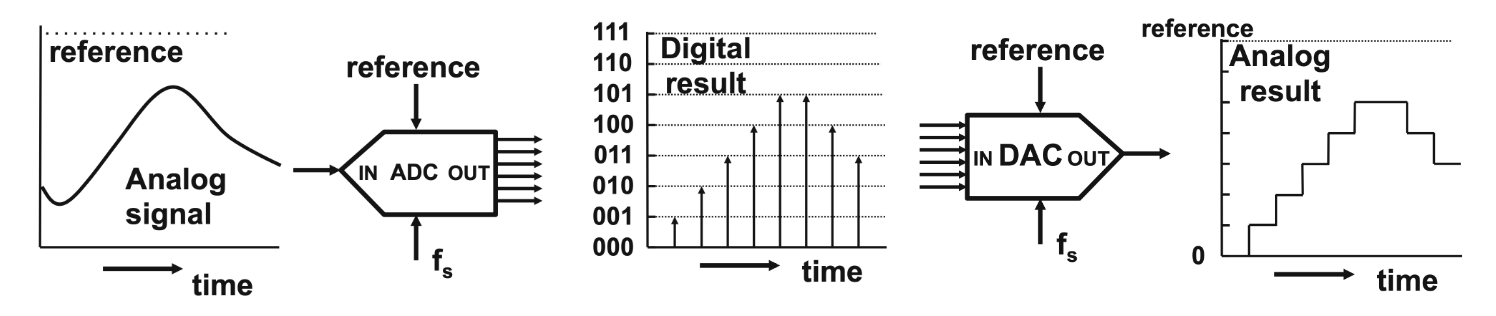
\includegraphics[width=0.7\linewidth]{img/ADC-DAC.png}
    \caption{\gls{adc} to \gls{dac} conversion}
  \end{center}
\end{figure}

\begin{wrapfigure}{r}{0.5\textwidth}
  \begin{center}
    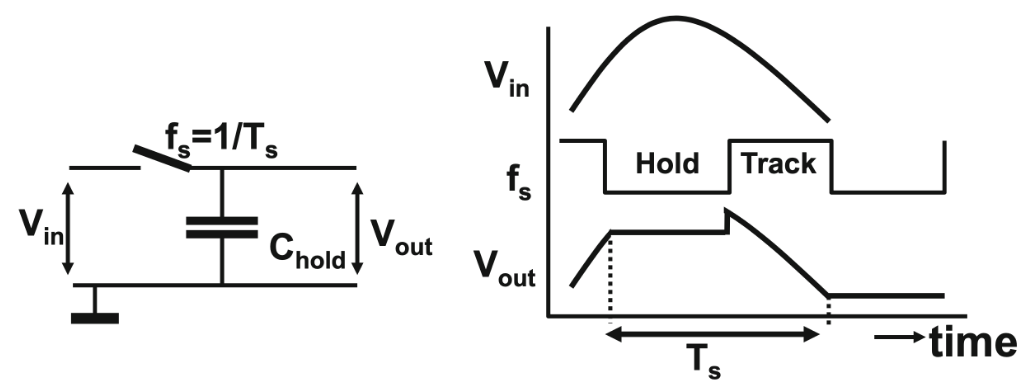
\includegraphics[width=0.95\linewidth]{img/th.png}
  \end{center}
  \caption{Track and Hold}
\end{wrapfigure}


And of course, going from digital to analog requires to do some amplitude restoration and holding the signal to make it continuous. Important to understand that the digital values only make sense if we have a sampling frequency and a reference voltage where $111...111 = V_{ref}$. So the binary number represents a fraction of this reference voltage.\\
To sample this we are using a \textit{Track and Hold} rather than a sample and hold since it is not quite easy to sample (opening the switch for a small small amount of time). Of course, this switch is implemented as a MOS transistor where we can take advantage of its symmetry to either charge or discharge the capacitance.\\
If we want to have a \textit{Sample and Hold} we can chain two track and hold back to back using inverted clocks. But it can be quite tricky to have such precision when designing the circuit.

\subsubsection{Requirements}

We want good \textit{speed}, so short tracking period and have a high bandwidth which implies to have a small $\tau$ (big switch, small cap). On the other hand, for accuracy we want to have a low noise ($\frac{kT}{C}$) so a big capacitance and low distortion so a linear switch. We can see this is a major trade-off in T\&H design.

\section{Non-idealities}

\subsection{Noise}

\begin{wrapfigure}{r}{0.33\textwidth}
  \begin{center}
    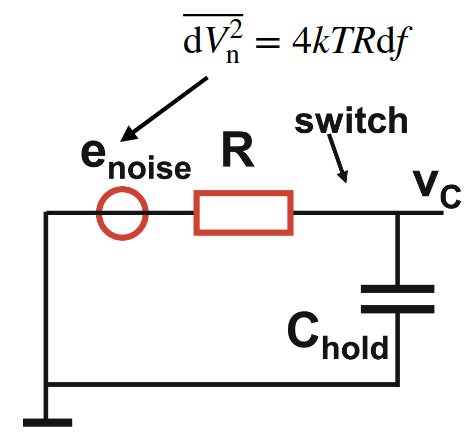
\includegraphics[width=0.95\linewidth]{img/noise_sampling_switch.png}
  \end{center}
  \caption{Noise in a sampling switch}
\end{wrapfigure}

We can represent the switch (implement as a transistor) with a resistor that has an equivalent noise source $e_{noise}$. Depending on the $C_{hold}$ value we will have various difference equivalent noise voltages:

\begin{align}
    v_{C,noise}^2 &= \int_{f=0}^{f=\infty} \frac{4kTR df}{1 + (2\pi f)^2R^2C^2} = \frac{kT}{C}\\
    SNR &= \frac{P_{signal}}{P_{noise}} = \frac{A^2/2}{kT/C}
\end{align}

Where $A/\sqrt{2}$ represents the RMS amplitude of the signal. It is interesting to notice how this noise is only present when we are having the switch high so theoretically no noise should be present in the hold phase.\\
Hence, this noise is also sampled ! Even though it will be flat for any frequency below Shannon and has a zero mean and variance of $\sigma = kT/C$. This will create some \textit{aliasing}. The noise PSD will \textbf{increase} due to sampling since we will have some shorter bandwidth (\textit{check this}).
\begin{align}
    S_{vv,RC} &= 4kTR = \frac{2kT}{\pi C f_{RC}} & S_{vv,s} &= \frac{2kT}{Cf_s}
\end{align}

What happens is the fact we have a noise density covering all possible frequencies which gets sampled and so we have a stack up of noise which is technically infinite. But since we have a capacitance and resistor that samples the signal and noise this will act as a low pass filter and will create some sorts of lobes. The \textbf{total sampled noise} is always $kT/C$.\\
The increase of noise spectral density depends on noise bandwidth and this causes problem for high-resolution converters. It is not always ideal to have a high bandwidth

\subsection{Jitter}

It is a form of \textit{statistical noise} and is due to noisy clock generator which won't sample reliably and will sometimes happen slightly before or after the "\textit{tick}". Jitter can be deterministic which will result in \textit{tones} in the spectrum or distortion for signal-dependent jitter (definition of what distortion is). We can find the result of $\sigma_t$ has on our sampled amplitude : 

\begin{align}
    A(t) &= A sin(\omega t) & \sigma_A^2(nTs) &= \left(\frac{dA(nTs)}{dt}\right)^2 \sigma_t^2 = \omega^2A^2 cos^2(\omega nT_s)\sigma_t^2\\
    A(nT_s+\Delta t(t)) &= A sin(\omega (nT_s + \Delta t(t)) & \sigma_A^2 &= \frac{\omega^2 A^2 \sigma_t^2}{2}\\ 
    \Delta A(nT_s) &= \frac{d A sin(\omega t)}{dt} \Delta t(nT_s) & \Delta A(nT_s) &=  \omega A cos(\omega nT_S)\Delta t(nT_s) 
\end{align}

The jitter acts as a sort of ceiling, to fight against the thermal noise we can simply increase the input voltage but at some point the SNR due to noise and jitter are equal and the SNR of jitter is the limit since it only depends on the frequency.

\subsection{Non fundamental error - Implementation error}

\subsubsection{Pedestal}

Pedestal error is linked with the charges in the channel \textbf{and} the parasitic cap $C_{ped}$ which goes from gate to source. There is some charges that once the switch is closed will get injected or removed.\\
One solution is the compensation circuit where we will use dummy switches which will take those extra charges. This requires a duty cycle of $50\%$ and precise clock to "capturate" those extra charges precisely.

\subsubsection{Droop}

The charges put on $C_{hold}$ may go down with time especially with BJT as the base will draw currents. It is linked with leakage : 

\begin{equation}
    V_{droop} = -\frac{I_{leak} T_{hold}}{C_{hold}}
\end{equation}

\subsubsection{Feedthrough}

 We also have a capacitance between the source and the drain which will cause a small current to \textit{feedtrhough}. One solution is to use \textbf{t-switch} which helps to reduce the effect. In differential implementations we can use some \textit{cross-coupled always-off} switches. 

 \subsubsection{Aperture Jitter}

We won't have a perfect instantaneous rise so the logic 1 or logic 0 may not appear exactly at the clock period.


\section{Capacitor and switch implementations}

\subsection{Capacitors}

In IC design we will mostly focus on \textbf{Metal-Insulator-Metal} (MIM) capacitor which requires a special process and are linear. The other type is the interconnect \textbf{MOM} which doesn't require a special process. One key idea is to create the capacitance as high as possible on the metal layers to get away from parasitic due to the wafer.\\

We can also do some \textit{vertical} MOM. This solution takes advantage of the height of the metal stack but the lower end will me more susceptible to parasitic and we use the other symbol of a capacitance.\\

It is sometimes hard to model capacitance due to the fact we have multiple field lines going and connecting with all the layers. So one trick is to isolate each capacitance and shield each one of them. It makes analysis much easier.

\subsection{Switches}

The switch (NMOS or PMOS) has its own $R_{on}$ which is proportional to $1/V_{in}$. We not only need a small enough resistor for good $\tau$ but also a constant one to avoid distortion !

\begin{align}
R_{o n, N M O S} & =\frac{1}{(W / L)_N \beta_{N \square}\left(V_{D D}-V_{i n}-V_{T, N}\right)} &
R_{o n, P M O S} & =\frac{1}{(W / L)_P \beta_{P \square}\left(V_{i n}-\left|V_{T, P}\right|\right)}
\end{align}

One idea to reduce this $\propto V_{in}$ is to use \textbf{complementary switches} so the NMOS and PMOS behavior will kinda cancel out. For this to work we need sufficient $V_{DD}$ namely $ V_{DD} < V_{th,n} + |V_{th,p}|$. We can boost V using some \textit{Cockroft-Walton multiplier} or \textit{Dickson multiplier}.

\subsubsection{Bootstrapping}

The idea behind bootstrapping is to keep the sample pulse and input voltage constant which will result in constant $R_{on}$.

\begin{figure}[H]
    \centering
    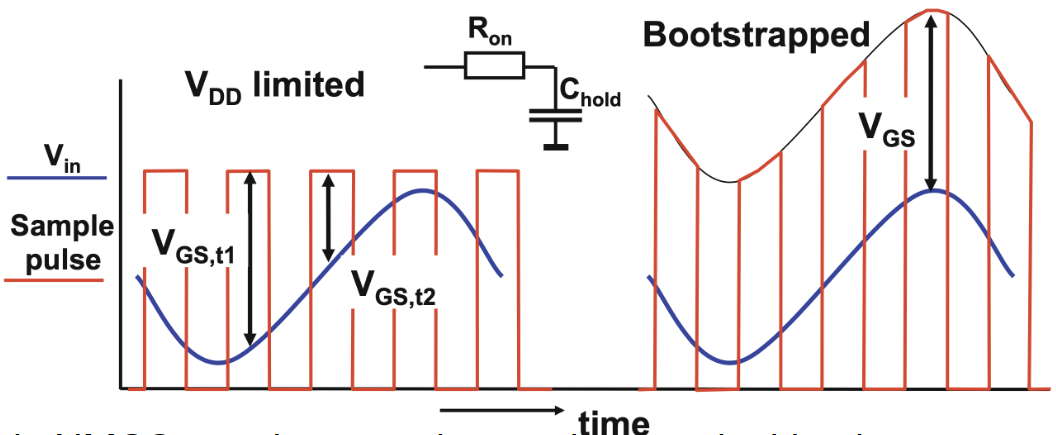
\includegraphics[width=0.5\linewidth]{img/bootstrapping.png}
    \caption{Bootstrapping}
    \label{fig:enter-label}
\end{figure}

Here we don't need to use two transistor, we can just use one NMOS and we get a high SNR for small $C_{hold}$. We keep the resistance constant and we don't have any distortion.\\
The main idea is to use a capacitance we charge to $V_{DD}$ in hold phase and when the tracking phase come the $V_{in}$ is added on top of the $V_{DD}$ that is stored on the cap making the $V_{gs} = V_{DD}$.\\

Some challenges we can face are voltage limit across the gate, drain and source. We also have a body diode which can create charge lost, latch-up or even current to substrate.

\begin{figure}[H]
    \centering
    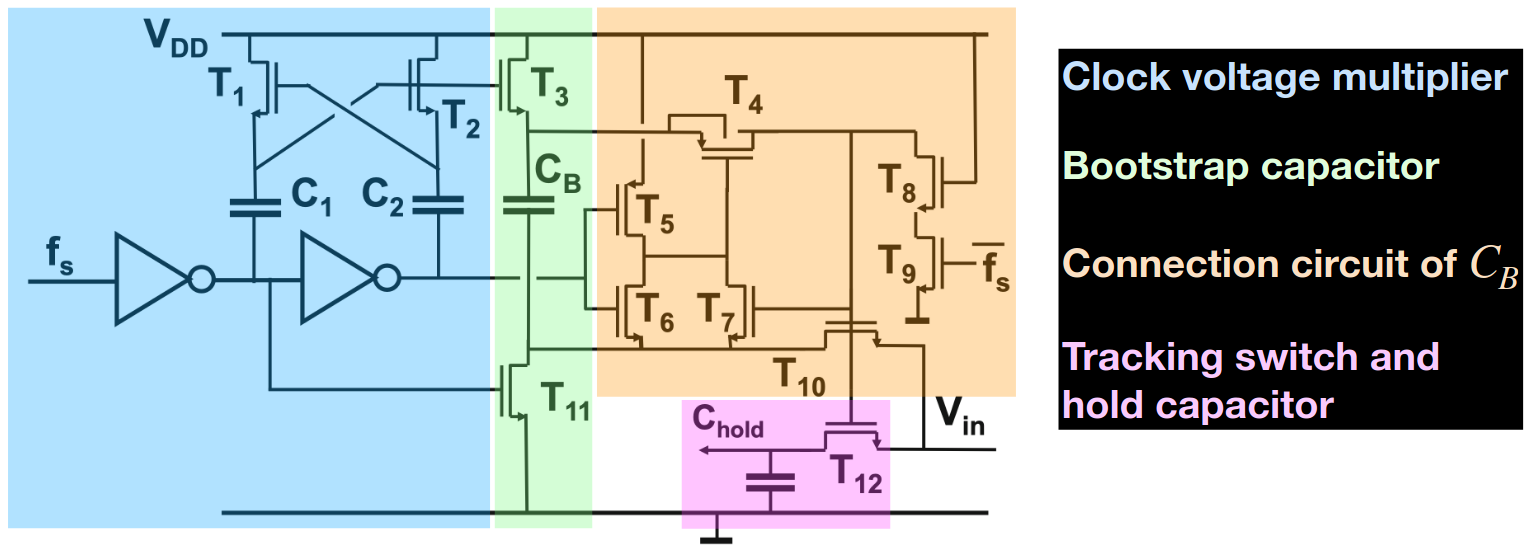
\includegraphics[width=0.75\linewidth]{img/typical_bootstrap.png}
    \caption{Typical bootstrap circuit}
    \label{fig:enter-label}
\end{figure}

We can also use a technique called \textit{bottom-plate sampling}. \textcolor{red}{add more info read a bit more about it}.

\section{Circuit topologies}

\subsection{General considerations}

We want to maintain the value on the capacitance, one solution is to use buffered implementation. Buffered implementation will be more accurate but we introduce a feedback system which inherently has delay thus some maximum possible speed.\\
We also need to keep in mind that when using a buffer (opamp) we will have an extra \textit{non-linear} capacitance in parallel with our hold capacitance. So we need to pick the right hold capacitance to minimize this extra non linear capacitance.\\
We always need to keep in mind what is this designed use for, what is the swing (rail-to-rail, buffer supply voltage above $V_{DD}$, ...).\\ 
High-gain opamp requires a low settling error $A_{DC} > \frac{1}{\epsilon} = 2^N$. The settling speed determnies unity-gain frequency of a track and hold buffer. the UGF palys a big role.

\subsection{Switched-capacitor T\& H circuits}

The most basic switched-cap implementation : 

\begin{figure}[H]
    \centering
    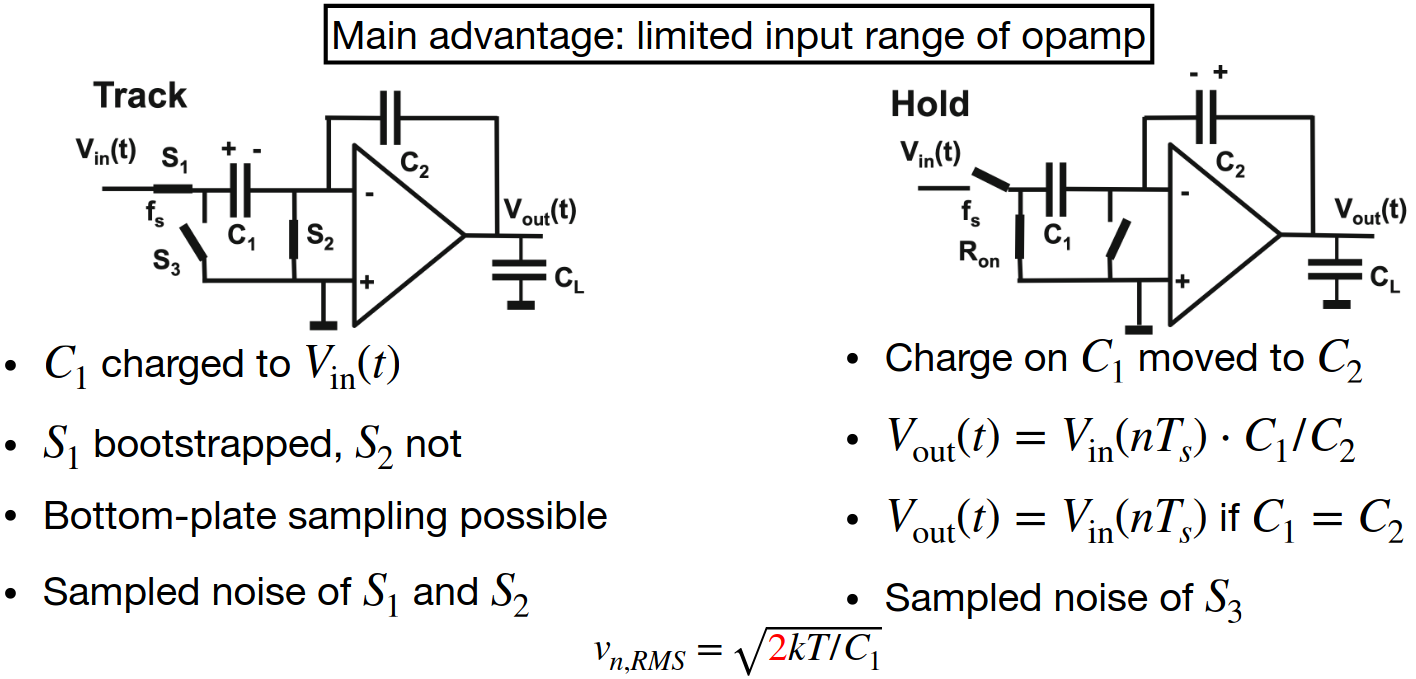
\includegraphics[width=1\linewidth]{img/basic_th_switched_cap.png}
    \caption{Basic Switched-cap implementation}
    \label{fig:basic-sc-label}
\end{figure}

In the \textit{track phase} we first discharge $C_2$. The $S_1$ is \textit{bootstrapped} and $C_1$ is charged to $V_{in}$. We have some sampled noise at $S_1$ and $S_2$. In the \textit{hold phase}, the charge from $C_1$ are moved to $C_2$ (charge recollection). We have $V_{out}(t) = V_{in}(nT_S) \cdot C1/C2$.\\

If we have \textit{unity-gain signal} we will have a $H = C_2/(C_1+C_2) = 1/2$ if $C_1 = C_2$. The closed loop gain is $A_{cl} = 2$ so we will amplify some unwanted signal. The setting time is determined by $1/2 \tau$.

\subsection{Flip-Around T\&H}

\begin{figure}[H]
    \centering
    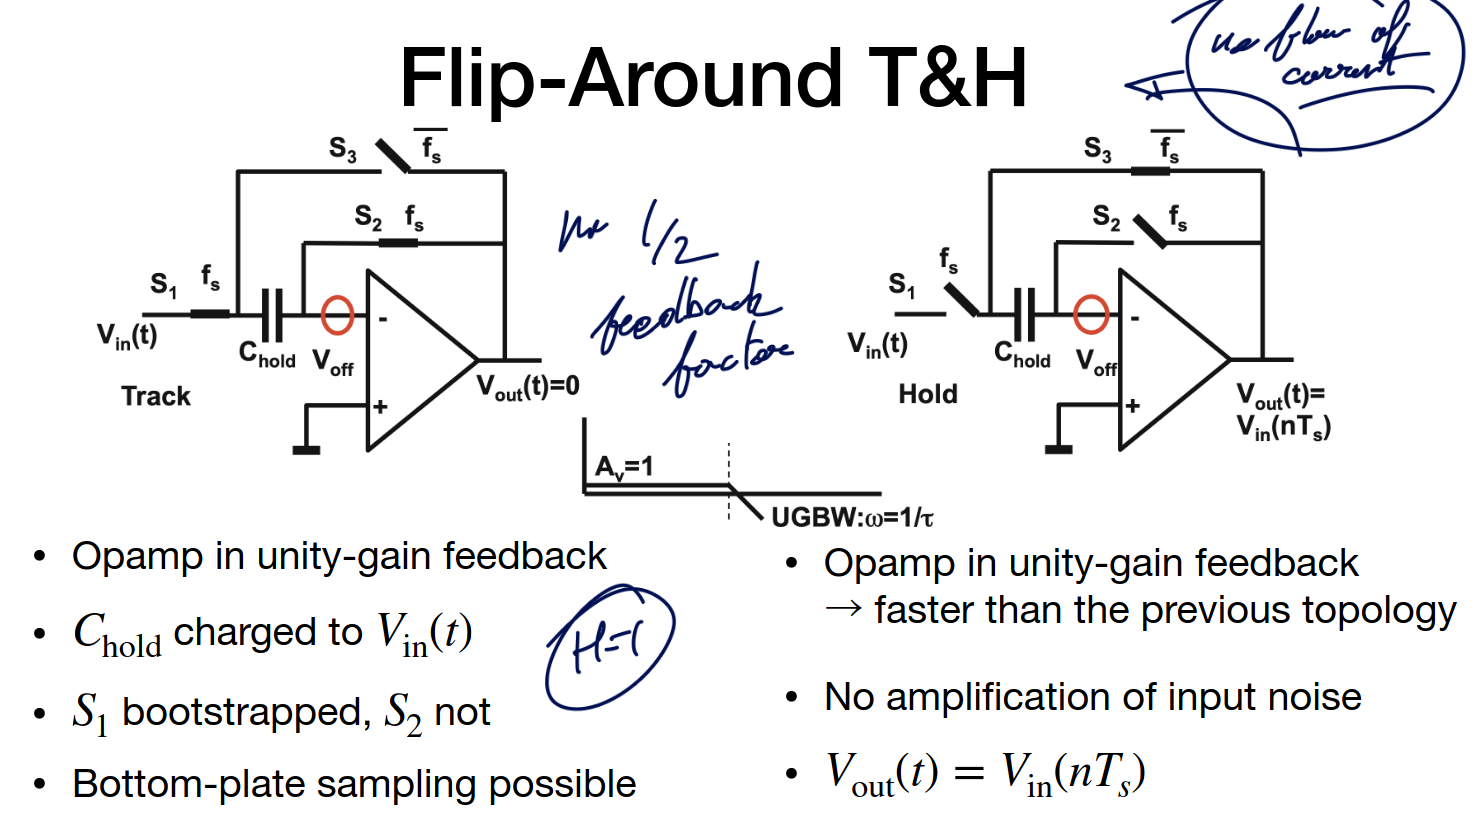
\includegraphics[width=0.75\linewidth]{img/Flip_around.png}
    \caption{Flip-Around track \& hold}
    \label{fig:flip-around-label}
\end{figure}

It will use a virtual ground to charge and discharge the cap. Here we have a unity-gain feedback of 1 which is desirable. But this virtual ground isn't perfect and so we will have some \textit{offset}. But this offset will actually be cancelled !

\begin{align}
    \text{Track mode : }& V_{C_{hold}} (nT_S) = V_{in}(nT_S) - V_{off} \\
    \text{Hold mode : }&  V_{out}((n+1/2)T_S) = V_{C_{hold}} (nT_S) + V_{off} = V_{in}(nT_S)
\end{align}

If we go in the z-domain to analyze this error we find : 

\begin{align}
    V_{out,error} &= V_{off} (z) (1-z^{-0.5})\\
    H(f) &= 2 sin(\pi f/2f_s)
\end{align}

So it will suppress the offset and the noise at low-frequency. But the high-frequency noise will be doubled and the sample noise on $C_{hold}$ is still present.

\begin{figure}[H]
    \centering
    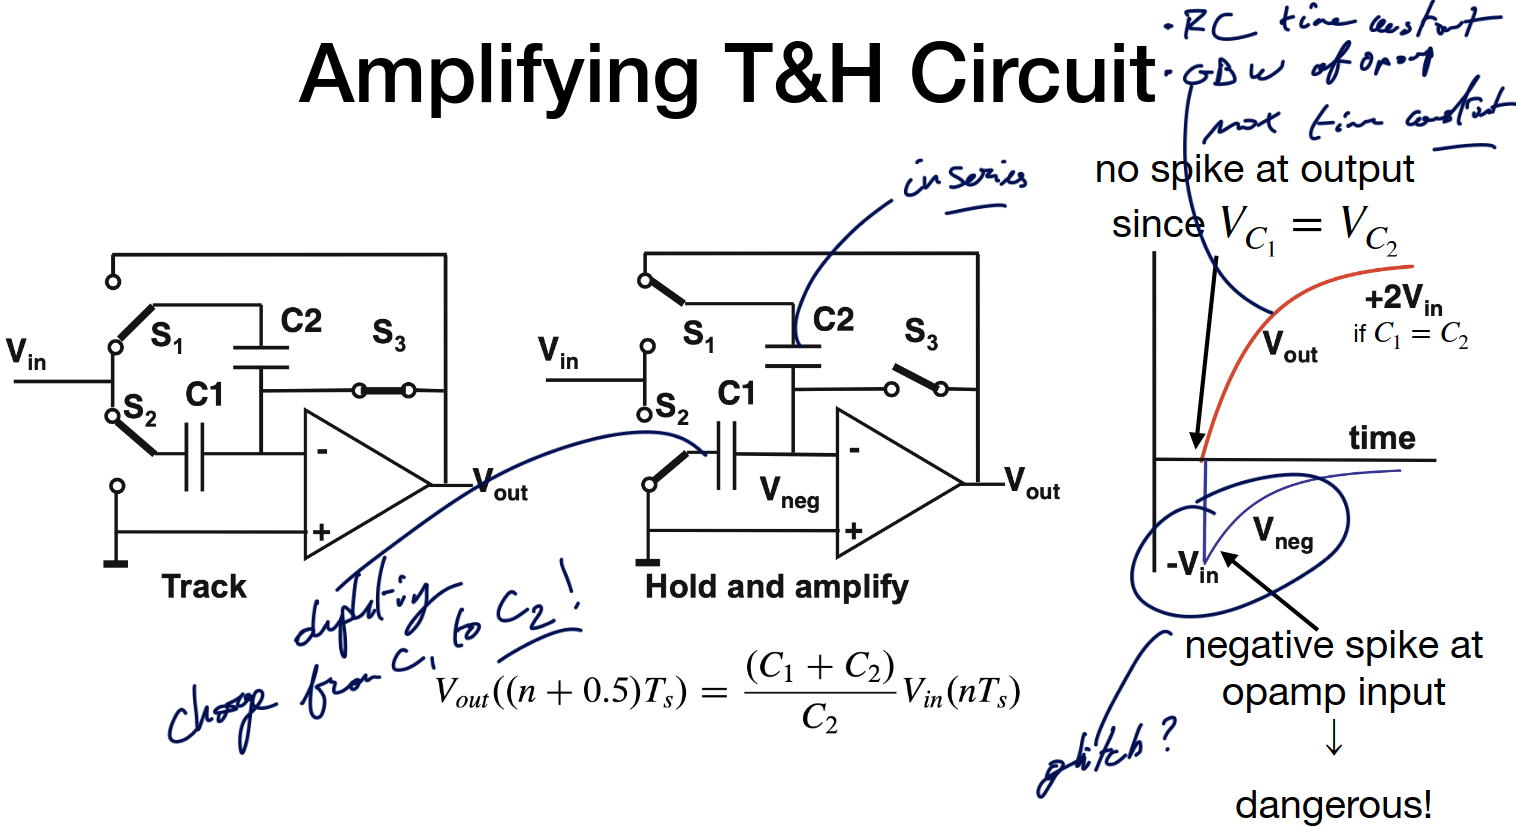
\includegraphics[width=0.75\linewidth]{img/Amplifying_Track.png}
    \caption{Amplifying track \& hold}
    \label{fig:amplifying-th-label}
\end{figure}

We can see some dangerous spikes on fig. \ref{fig:amplifying-th-label}. The noise can be found as follow :

\begin{align}
    v_{in,noise}^2 &= \frac{kT}{C_1+C_2} & v_{out,noise}^2 &= \frac{kT(C_1+C_2)}{C_2^2} + \text{noise OpAmp}
\end{align}

\subsection{Correlated double sampling}

In sensors and and image sensor we want to get rid of those unwanted component. Often, we will have 2 samples time where we will first get a baseline then the actual signal we want to remove the offset component.

\begin{figure}[H]
    \centering
    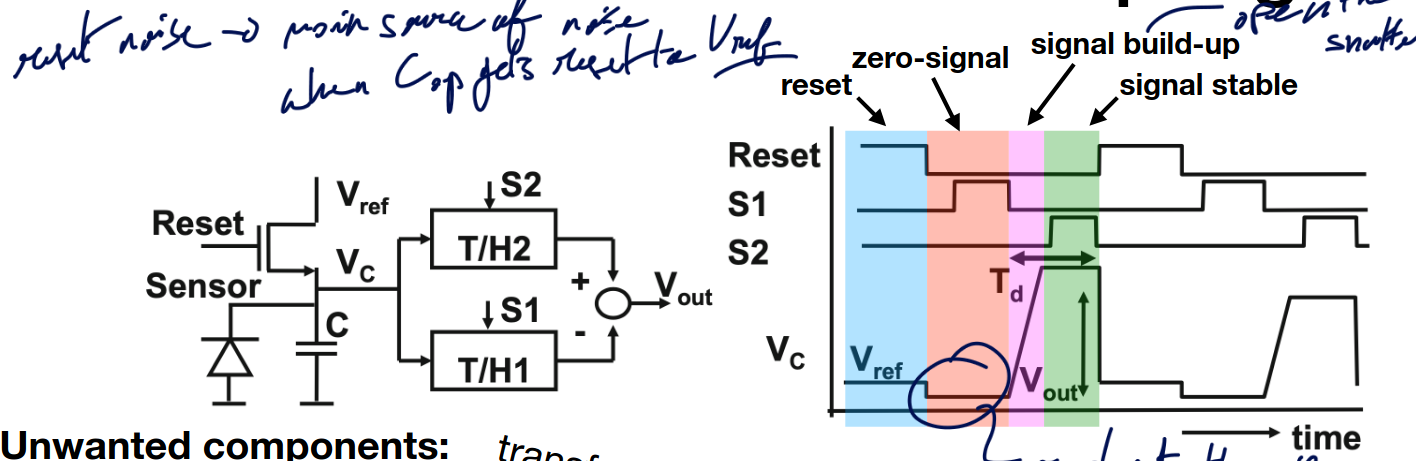
\includegraphics[width=0.75\linewidth]{img/double_corr.png}
    \caption{Correlated double sampling}
    \label{fig:double-correlated-label}
\end{figure}

\begin{align}
    |H(s)| &= |1 - e^{-sT_d}| = |e^{-sTd/2}| = |e^{-sT_d /2} 2 sin(sT_d /2) |\\
    |H(\omega)| &= |2sin(\omega T_d / 2)| = |2 sin(\pi f T_d)|
\end{align}

It will reject the low-frequency noise but will \textit{amplify} by $1/2T_d$ the noise near \textit{odd multiples}.

\chapter{Digital-to-Analog Conversion}

We need to differentiate two different use cases of a \gls{dac} namely :

\begin{enumerate}
    \item \underline{Convert to physical domain :} when we need a \textit{high quality} at every time instant. We need a minimum amount of power to be able to draw some current. For example a USB-C to jack adapter !
    \item \underline{Generate reference value for an \gls{adc} :} typically needed in a SAR \gls{adc}. We only need this conversion at some specific point in time and the drive capabilities are not exigent.
\end{enumerate}

\section{Signal representations}

\begin{itemize}
    \item \underline{Straight binary:} only positive signals
    \item \underline{Two’s complement:} easy addition and subtraction, zero signal at half reference (noisy!)
    \item \underline{Sign and magnitude:} no noisy half reference values for zero signal, digital decoder needed, simple rounding results in cross-over distortion
    \item \underline{Gray coded:} only one bit changes
\end{itemize}

\begin{table}[H]
    \centering
    \begin{tabular}{|c|c|c|c|c|c|c|c|}
        \toprule
        \multicolumn{2}{c|}{\textbf{Straight binary}} & \multicolumn{2}{c|}{\textbf{Two’s complement}} & \multicolumn{2}{c|}{\textbf{Sign+magnitude}} & \multicolumn{2}{c|}{\textbf{Gray coded}} \\
        \midrule
        15 & 1111 & 7  & 0111 & 7  & 0111 & 15 & 1000 \\
        14 & 1110 & 6  & 0110 & 6  & 0110 & 14 & 1001 \\
        13 & 1101 & 5  & 0101 & 5  & 0101 & 13 & 1011 \\
        12 & 1100 & 4  & 0100 & 4  & 0100 & 12 & 1010 \\
        11 & 1011 & 3  & 0011 & 3  & 0011 & 11 & 1110 \\
        10 & 1010 & 2  & 0010 & 2  & 0010 & 10 & 1111 \\
        9  & 1001 & 1  & 0001 & 1  & 0001 & 9  & 1101 \\
        8  & 1000 & 0  & 0000 & 0  & 0000 & 8  & 1100 \\
        7  & 0111 & -1 & 1111 & 0 & 1000 & 7  & 0100 \\
        6  & 0110 & -2 & 1110 & -1 & 1001 & 6  & 0101 \\
        5  & 0101 & -3 & 1101 & -2 & 1010 & 5  & 0111 \\
        4  & 0100 & -4 & 1100 & -3 & 1011 & 4  & 0110 \\
        3  & 0011 & -5 & 1011 & -4 & 1100 & 3  & 0010 \\
        2  & 0010 & -6 & 1010 & -5 & 1101 & 2  & 0011 \\
        1  & 0001 & -7 & 1001 & -6 & 1110 & 1  & 0001 \\
        0  & 0000 & -8 & 1000 & -7 & 1111 & 0  & 0000 \\
        \bottomrule
    \end{tabular}
    \caption{Binary Representations}
    \label{tab:binary}
\end{table}

To represent those bits in hardware we can go either for the \textit{thermometer} or \textit{binary} representation. In the thermometer representation each cells are of the same size and to increase numbers we need to increase the amount of cells on. It grantees \textbf{monotonicity}. For the binary, they are not of equal size but has the advantage to need $n$ for $n$ bits while it is $2^n$ cells for thermometer. It is not guaranteed to be monotonic and the large switch of cells can create glitches.\\

We can also use \textit{segmentation} to leverage from both type of implementation.

\begin{table}[H]
    \centering
    \renewcommand{\arraystretch}{1.3} % Adjust row height
    \begin{tabular}{|l|c|c|}
        \hline
        \textbf{Architecture} & \textbf{Unary} & \textbf{Binary} \\
        \hline
        Monotonicity & By design & Not guaranteed \\
        \hline
        Number of elements & $\propto 2^N$ & $\propto N$ \\
        \hline
        Area, parasitics & $\propto 2^N$ & $\propto N$ \\
        \hline
        \gls{inl} systematic & Gradient & Small \\
        \hline
        \gls{inl} random & $\propto \sigma_{element} \sqrt{2^N-1}$ & Same with \gls{dnl} errors \\
        \hline
        \gls{dnl} random & $\propto \sigma_{element}$ & $\propto \sigma_{element} \sqrt{N, \dots, 2^N-1}$ \\
        \hline
        Switching energy & $\propto$ Signal & Can be large and non-linear \\
        \hline
        Decoder complexity & $2^N$-to-1 & Simple \\
        \hline
        Power & \multicolumn{2}{c|}{Choice for R, I, or C implementation dominates power} \\
        \hline
        Noise & \multicolumn{2}{c|}{Similar for similar power levels} \\
        \hline
    \end{tabular}
    \caption{Comparison between Unary and Binary Architectures}
    \label{tab:unary_vs_binary}
\end{table}

We need to keep in mind that the \gls{dnl} is the difference between one step to the other and it must be lower than $1 LSB$. The \gls{inl} is the integrate error and so cumulate the error. Those issues will lead to distortion and harmonics !

\subsection{Typical \gls{inl} of Unary Architectures}

Here we have $A_{lsb}$ that represents the minimum voltage we can add so the minimum cell. To represents a number and it's unused counter part : 

\begin{align}
    y_1 &= \sum_{i=0}^{m-1} A_{lsb}(i) \quad \mathbb{E}(y_1) = m A_{lsb} \quad \sigma_{y_1} = \sigma_{A_{lsb}} \sqrt{m}\\
    y_2 &= \sum_{i=m}^{2^N-1} A_{lsb}(i) \quad \mathbb{E}(y_2) = (2^N-m) A_{lsb} \quad \sigma_{y_2} = \sigma_{A_{lsb}} \sqrt{2^N -m}
\end{align}

To find the \gls{inl} we can use this formula \textbf{WHY THIS FORMULA I DON4T GET IT ???}

\begin{align}
    INL(m) &= \frac{2^N \sum_{i=0}^{m-1} A_{lsb}(i) }{\sum_{i=0}^{2^N - 1} A_{lsb}(i) } - m = \frac{2^N y_1}{y_1 + y_2}  - m\\
    \sigma_{INL}^2(m) &= \left(\frac{\partial INL(m)}{\partial y_1} \right)^2 \sigma_{y_1}^2 + \left(\frac{\partial INL(m)}{\partial y_2} \right)^2 \sigma_{y_2}^2\\
    &= \left( \frac{y_2}{(y_1+y_2)^2} \right)^2 m \sigma_{A_{lsb}}^2 + \left( \frac{-y_1}{(y_1+y_2)^2} \right)^2 (2^N-m) \sigma_{A_{lsb}}^2\\
    &= \frac{m(2^N - m)}{2^N} \frac{\sigma_{A_{lsb}}}{A_{lsb}^2}
\end{align}

\subsubsection{Segmented cells}

\begin{figure}[H]
    \centering
    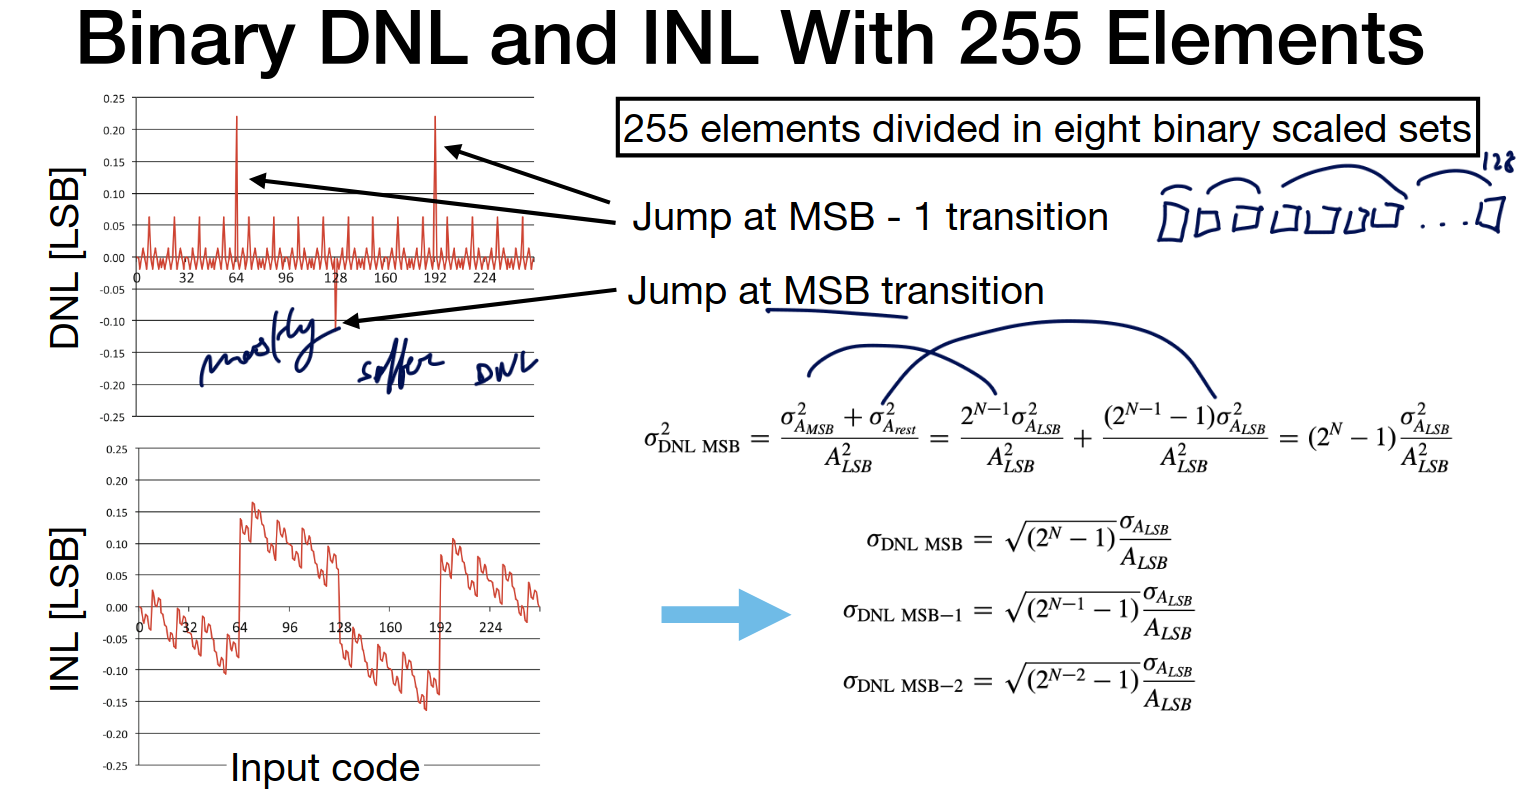
\includegraphics[width=0.75\linewidth]{img/segmented_DNL_INL.png}
    \caption{Segmented \gls{dnl} and \gls{inl}}
    \label{fig:segmented-cell-label}
\end{figure}

The less binary scaled elements we have the stronger those jumps and glitches will be. It may even lead to \gls{dnl} being over $1$ LSB meaning we can't guarantee monotonicity anymore this will result in missing code.

\begin{equation}
    \sigma_{DNL, MSB} = (2^N -1) \frac{\sigma_{A_{lsb}}}{A_{lsb}}
\end{equation}

\begin{table}[H]
    \centering
    \renewcommand{\arraystretch}{1.3} % Adjust row height
    \begin{tabular}{|l|c|c|}
        \hline
        & \textbf{Unary} & \textbf{Binary} \\
        \hline
        Voltage & Resistor string & R-2R \\
        &  \textit{Flash \gls{adc}} & \textit{Low-performance \gls{dac}} \\
        \hline
        Current & Current matrix & Current splitting \\
        &  \textit{High bandwidth \gls{dac}} & \\
        \hline
        Charge/capacitor & Capacitor bank & Capacitor bank \\
        &  \textit{Low power \gls{dac}} & \\
        \hline
        Time & PWM, $\Sigma\Delta$ mod &  Limited by distortion \\
        &  \textit{Low bandwidth \gls{dac}} & \\
        \hline
    \end{tabular}
    \caption{Comparison of Unary and Binary Architectures, \gls{dac} and \gls{adc}}
    \label{tab:unary_binary_comparison}
\end{table}

\section{Digital-to-analog conversion}

\subsection{Voltage domain}

\subsubsection{Resistor ladder}

The simplest \gls{dac} we can think of is a \textbf{resistive ladder} where we use a thermometer code based approach. We need $2^N$ resistors between $V_{ref+}$ and $V_{ref-}$. We need a buffer to drive the load so we don't have some currents that flow back into the resistive ladder which would cause some monoticity and values change. This buffer op-amp isn't straightforward as it needs to be a rail-to-rail op-amp.\\

The equivalent input impedance seen by the input of the buffer is given as :

\begin{equation}
    R_{eq} (m) = \frac{\frac{m}{2^N} R_{tot} \cdot \frac{2^N-m}{2^N} R_{tot} }{\frac{m}{2^N} R_{tot} + \frac{2^N-m}{2^N} R_{tot}} = \frac{m(2^N-m)}{2^{N+1}} R_{tot}
\end{equation}

We have a signal-dependent current delivery and the resistor is parabolic. Due to the capacitive load we also have a signal-dependent time constant. This lead to distortion at high frequencies.

\begin{align}
    V(m) &= \frac{m}{2^N} V_{ref} = \frac{mR}{mR + (2^N -m)R} V_{ref} = \frac{R_1}{R_1 + R_2} V_{ref}\\
    \sigma_{V}^2(m) &= \left( \frac{\partial V(m)}{\partial R_1} \right)^2 \sigma_{R_1}^2  + \left( \frac{\partial V(m)}{\partial R_2} \right)^2 \sigma_{R_2}^2 \\
    &= \left( \frac{R_2}{(R_1+R_2)^2} \right)^2 \sigma_{R_1}^2 V_{ref}^2  +  \left( \frac{-R_1}{(R_1+R_2)^2} \right)^2 \sigma_{R_2}^2 V_{ref}^2\\
    &= \frac{m(2^N -m)}{2^N} \frac{\sigma_R^2}{R^2} \frac{V_{ref}^2}{2^{2N}} =  \frac{m(2^N -m)}{2^N} \frac{\sigma_R^2}{R^2} V_{LSB}^2\\ 
    \sigma_{INL}^2 &= \frac{m(2^N- m)}{2^N} \frac{\sigma_R^2}{R^2}
\end{align}

\textbf{ADD MORE INFO}

\subsubsection{R-2R ladder}

\begin{figure}[H]
    \centering
    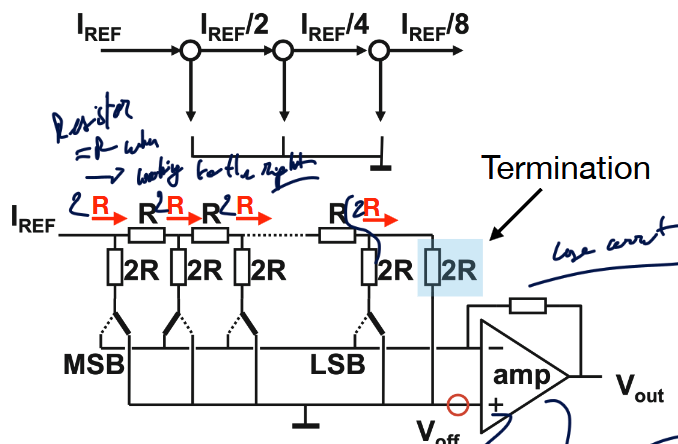
\includegraphics[width=0.75\linewidth]{img/R_2R.png}
    \caption{R-2R Ladders}
    \label{fig:R-2R-label}
\end{figure}

Here we are using a binary structure and we only need a $2N$ resistors. It is not super precise since we have a lower and lower current flowing in each branch which will be more susceptible to noise. The accuracy depends on :

\begin{enumerate}
    \item \underline{Offset voltage :} non-ideal virtual ground and so we have some error in the current split. $V_{off} < \frac{I_{REF} R}{2^N}$.
    \item \underline{Resistor matching :} we need good matching or we will have large difference.
    \item \underline{Switch resistance :} the switch will add some $R_{on}$ resistance so we need it to be small to have a small impact.
\end{enumerate}

\subsubsection{Segmented resistor ladder}

\begin{figure}[H]
    \centering
    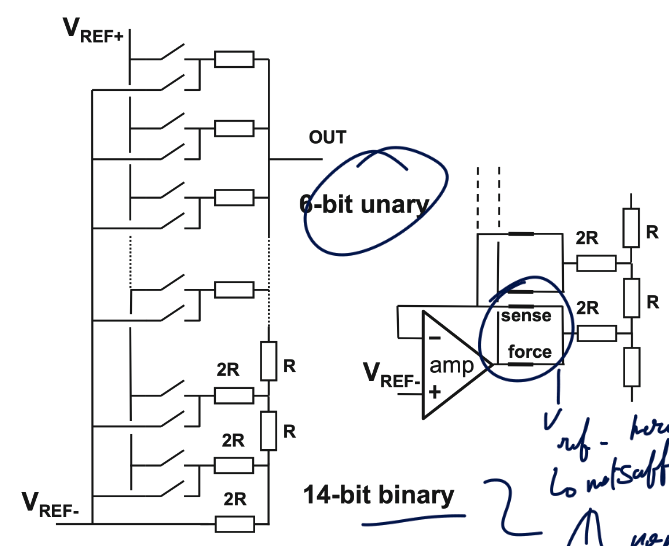
\includegraphics[width=0.75\linewidth]{img/segmented_r_ladder.png}
    \caption{Segmented resistor ladder}
    \label{fig:segmented-resistor-label}
\end{figure}

We will have a thermometer and binary part. It will improve the precision. There is no current in sense path. The sense node is equal to $V_{ref}$. We calibrate this offset voltage and we can also call it a \textit{kelvin contact} or \textit{four-point sensing}.

\subsection{Current domain}

Here instead of using resistor that will drive another resistor creating a voltage that gets buffered, we will directly work with current source that will drive a resistor which will have its voltage buffered. We can either go for a thermometer or binary coded version : 

\begin{figure}[H]
    \centering
    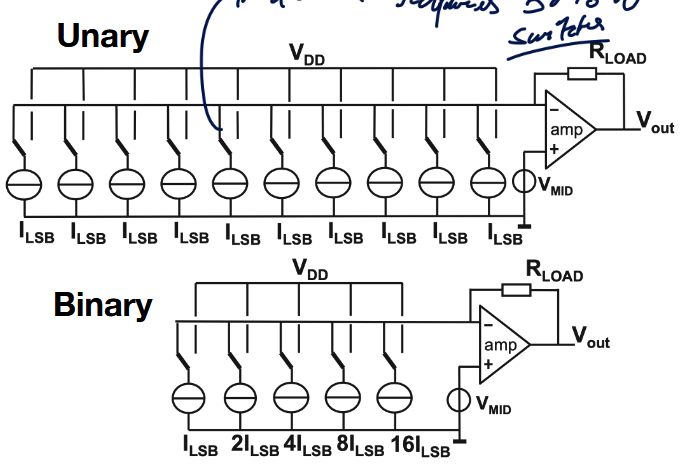
\includegraphics[width=0.65\linewidth]{img/Buffered_Current_DAC.png}
    \caption{Buffered Current \gls{dac}}
    \label{fig:enter-label}
\end{figure}

We need to keep all current source on even if they are not used to avoid \textit{current dump}. The amplifier is sensing the current so we call it a \gls{tia}. We need a low input impedance to limit the swing and low output one so we can drive any type of load.

\subsubsection{Symmetrical Buffered current-DAC}

\begin{figure}[H]
    \centering
    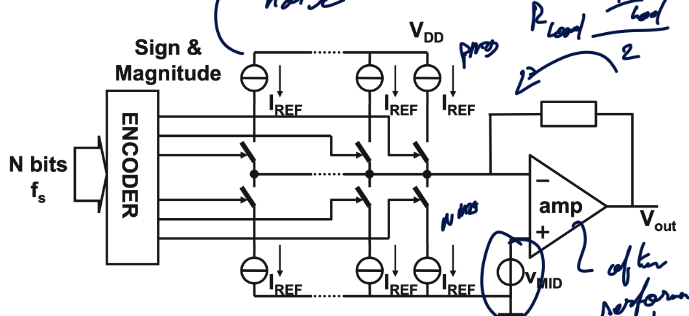
\includegraphics[width=0.75\linewidth]{img/sym_dac.png}
    \caption{Symmetrical buffered current-DAC}
    \label{fig:sym-buffered-DAC-label}
\end{figure}

To avoid some important switching (on and off) due to the representation of a number in signed format, we want to use a symmetrical one. Since most of the signal will be around 0 often going positive and negative. This configuration will reduce the 1/f and thermal noise. Here we need a current sink and current source so a NMOS and PMOS network is required (may be a designed constraint and we need to match PMOS and NMOS). We only have the noise of the buffer for zero level. We will need some calibration to manage a  balance between NMOS and PMOS.

\subsubsection{Buffer-less current-DAC}

\begin{figure}[H]
    \centering
    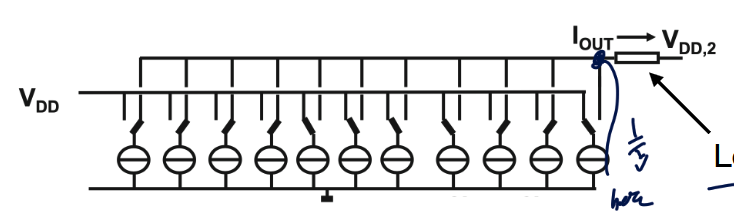
\includegraphics[width=0.75\linewidth]{img/bufferless_current_dac.png}
    \caption{Buffer-less Current DAC}
    \label{fig:BLC-DAC-label}
\end{figure}

Since we are not using a buffer, we have theoretically a larger bandwidth since we are not limited by the spec of a \gls{tia}. But in life there is always parasitic and so we will have a pole determined by the output load impedance and capacitance. It is a good choice for time-continuous signals with a matched impedance between $50-75\Omega$.

\subsubsection{Segment current DAC}

Based on the same idea of a buffer-less DAC we can use some current source that are $2^a$ LSB and some binary based sources starting at 1. This is segmenting and we use the thermometer for MSB part and the binary for the LSB as they take less space. The biggest issue is when we switch off binary section and we switch to the next unary source : 

\begin{figure}[H]
    \centering
    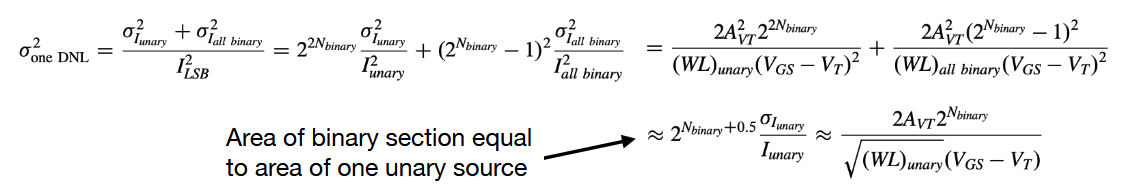
\includegraphics[width=0.95\linewidth]{eq_segme.png}
\end{figure}

We can also go further and add an extra rail to create current divider. This third rail will \textit{steer} unary current to current divider. The divider can be unary or binary scaled but we will have large transition error at the edge that will be reduced.

\subsubsection{Matrix decoding}

\begin{wrapfigure}{r}{0.5\textwidth}
    \centering
    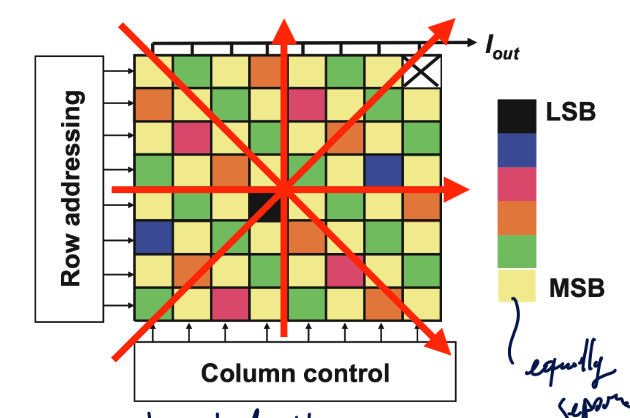
\includegraphics[width=1\linewidth]{img/centroid_layout.png}
    \caption{Centroid layout}
    \label{fig:centroid-layout-label}
\end{wrapfigure}

Usually in VLSI we will arrange thermometer current source in a matrix format so we can simply and quickly access the current. But due to the spreading of those current sources, we will accentuate some physical phenomena such as \textit{oxide thickness, power delivery drop, clock timing, temperature, ...} which will make the current sources unequal.\\

One technique to reduce this effect is presented on figure \ref{fig:centroid-layout-label}. We create symmetry in both direction and we will get rid of any \textbf{linear gradient}. We can go even further with some $Q^2$ walk and distributed subcell across the complete array or even use some \textit{randomize current cell} from one sample to the next (more advanced).\\

Some calibration we can make is \textbf{current source sorting} where we will measure all of the cells and create a sort of pair where we trigger a larger cell with a smaller one after. But we need a lot of pre-processing and measurements and we need to create some special metal routing over the cells which can deteriorate the performances even more. We also need into account possible delay and timing issues, ...

\subsubsection{Current cell implementation}

\begin{wrapfigure}{r}{0.5\textwidth}
    \centering
    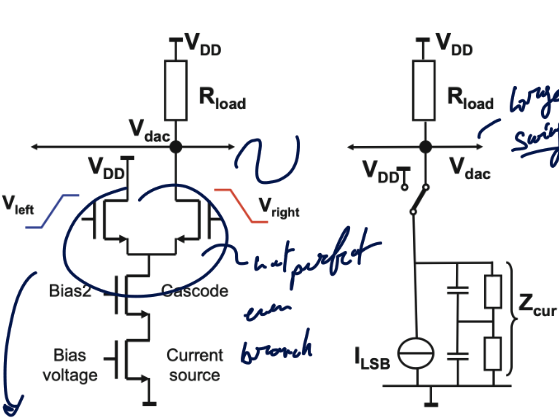
\includegraphics[width=0.95\linewidth]{img/current_cell.png}
    \caption{Current cell}
    \label{fig:current-cell-label}
\end{wrapfigure}

We keep the current source on to avoid distortion and keep the power consumption constant. The $V_{dac}$ will have considerable voltage variation which will create distortion.\\

Ideally the voltage drop is : 

\begin{align}
    V_{DD} - V_{dac} &= \alpha 2^N I_{LSB} R_{load}\\
    I_{err} &= \alpha Z^N V_{dac} / |Z_{cur}|
\end{align}

But we have a real voltage drop of :

\begin{align}
    V_{DD} - V_{dac} &= R_{load} \left( \alpha 2^N I_{LSB} + \frac{\alpha 2^N V_{dac}}{|Z_{cur}|} \right)
\end{align}
\begin{align}
    V_{dac} &= \frac{V_{DD} - R_{load} \alpha 2^N I_{LSB}}{1 + \alpha 2^N R_{load} / |Z_{cur}|}\\
    &\approx (V_{DD} - R_{load} \alpha 2^N I_{LSB}) \left( 1- \frac{\alpha 2^N R_{load}}{|Z_{cur}|}  + \left( \frac{\alpha 2^N R_{load}}{|Z_{cur}|} \right)^2 \right)
\end{align}

We will have a HD3 with $((2^N R_{load})/(4|Z_{cur}|))^2$

\subsubsection{Switch implementation}

\begin{wrapfigure}{r}{0.3\textwidth}
    \centering
    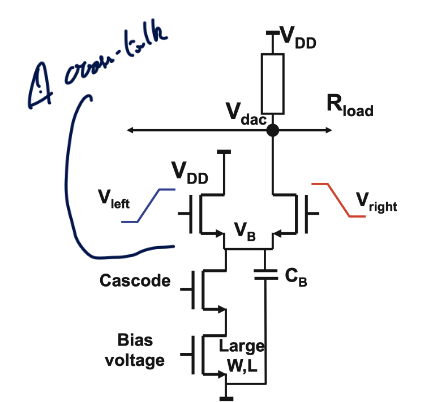
\includegraphics[width=0.9\linewidth]{img/switch_impl.png}
    \caption{Switch implementation}
    \label{fig:switch-impl-label}
\end{wrapfigure}

Switches are controlled by low-swing differential pulses to reduce cross-talk and minimize the creation of an inversion charge. We need to minimize the $V_B$ to have extremely accurate timing of switches. There is some charge taken from or released in output node at every switching event. Glitches are problematic for time-continuous output.\\

Architecture of choice for most demanding applications. We have a constant (high) power consumption and need a high-frequency clock and decoding logic require significant power. Differential implementation to cancel second-order distortion (big advantage). First-order relationship between linearity and bandwidth.

\subsection{Charge domain}
\subsection{Time domain}

\section{Accuracy improvement methods}

\chapter{Nyquist ADC}

This chapter will focus essentially about the comparator and will only cover some techniques applicable to Nyquist ADC.

\section{Comparator}

\section{Comparator}

\subsection{Requirements and operation principle}

A good starting point is to first summarize what we will need for this comparator block. Typically we want to measure and decide what an analog value should be in digital. So we will have to go from mV to V and be capable to be quite fast which means a good \gls{bw}. We have to be quite accurate while not using too much power and be able to measure and transform a wide range of signal. We must also ensure to always have a clear decision (no metastability) and no memory effect. So quite challenging.

\subsubsection{Limiting Amplifier}

We could think of chaining multiple amplifier but this can be quite slow and have some memory effect due to loss of inversion charge at output stages.

\begin{equation}
    V_{out}(t) = A^M V_{in}(t=0) \left[ 1 - e^{-t/\tau} \sum_{i=1}^{M} \frac{(t/\tau)^{i-1}}{(i-1)!} \right] \approx A^M V_{in}(t=0) \sum_{i=1}^{M} \frac{(t/\tau)^{i}}{(i-1)!}.
\end{equation}

\subsubsection{Latch behavior circuits}

We can also have some circuit that have a small feedback path which will create a hysterisis. It will first pre-amplify the small input signal and the positive feedback stage is activated to regenerate the still-small signal quickly.

\begin{figure}[H]
    \centering
    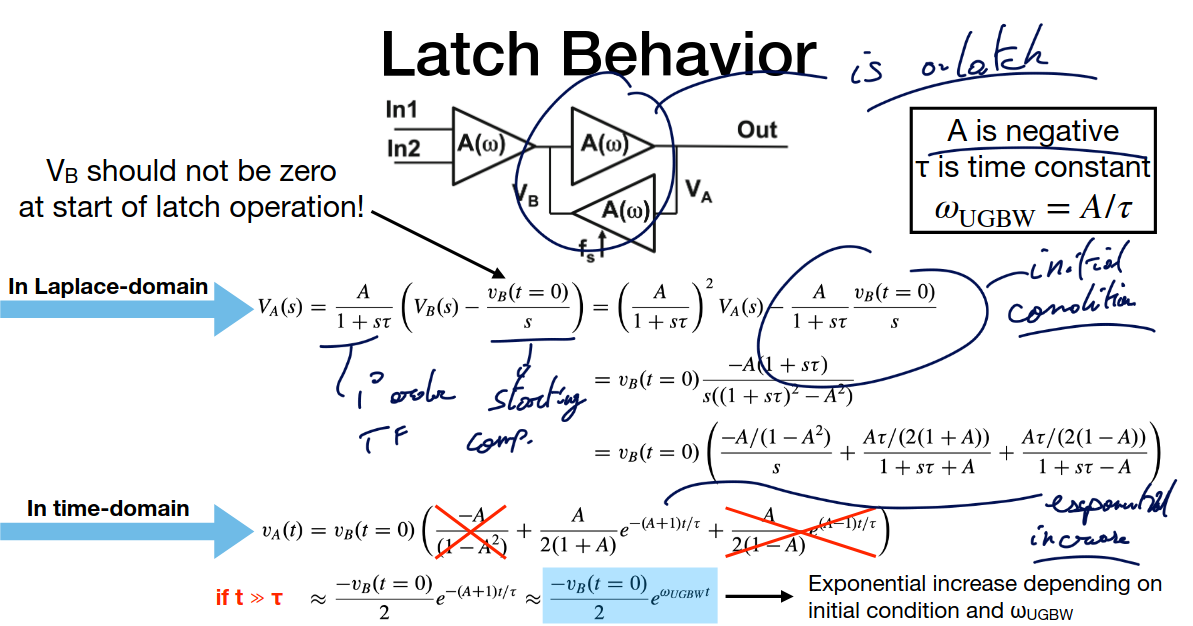
\includegraphics[width=0.75\linewidth]{latch_behavior.png}
    \caption{Latch behavior}
    \label{fig:enter-label}
\end{figure}


\subsection{Non-idealities}
\subsection{Comparator circuit examples}

\section{Analog-to-digital converter topologies}
\section{Conclusions}

\chapter{Delta Sigma \gls{adc}}

\section{Basic principles}

\begin{table}[H]
    \centering
    \begin{tabular}{|c|m{7cm}|}
        \hline
         Term & Definition  \\
         \hline
         Input sampling rate & Frequency at which the analog input is sampled\\
         \hline
         Output data rate & Frequency at which updated output words are available\\
         \hline
         Conversion gain & Ratio of an output amplitude over the input amplitude \\
         \hline
         Bandwidth & Frequency span in which the amplitude of an output sine is less then 3dB lower as the input amplitude, given a 1:1 conversion gain\\
         \hline
         \gls{snr} & // \\
         \hline
         \gls{enob} & Error free signal resolution $=(SNDR-1.76\text{ dB})/(6.02 \text{ dB})$\\
         \hline
    \end{tabular}
    \caption{Quick recap of definitions}
    \label{tab:my_label}
\end{table}

All those values are important metric when specifying an \gls{adc} but they can be misleading. We can trick the reader that we achieved exceptional result with a mediocre implementation. In fact We could find a hugeeee \gls{snr} if we filter the noise at the input 5 times lower than the nyquist frequency and then claim a figure that is $\sqrt{5}$ better than what we would truly have.

\subsection{\gls{fom}}

There is two main type of \gls{fom} used for \gls{adc} : 

\begin{enumerate}
    \item \underline{Schreier :} It is based on a theoretical idea and on information theory. We have a signal power and a maximum efficiency. It is based on the \textit{fundamental tradeoff} between accuracy and bandwidth, noise and power. But a critique that can be made is the fact it only uses \gls{snr} and not the \gls{sndr} which take into account more realistic issue. 
    \begin{align}
    P_{sig,min} &= 8kT \cdot BW \cdot SNR & \text{Power efficiency} &= \frac{P_{circuit}}{P_{sig,min}} = \frac{P_{circuit}}{8kT \cdot BW \cdot SNR}\\
    FoM &= 10^{10} log\left( \frac{SNR\cdot BW}{P_{ADC}} \right) & &=SNR (dB) + 10^{10} log\left( \frac{BW}{P_{ADC}} \right)
    \end{align}\\
    \item \underline{Walden :} It takes into account the \gls{sndr} and also use the bandwidth instead of only using the Nyquist frequency. So a more band limited \gls{fom}. The \gls{fom} is in Joule per conversion step.
    \begin{align}
        FoM &= \frac{Power}{2^{ENOB} \cdot min(2BW,f_s)}
    \end{align}
\end{enumerate}

There is also an issue related to the actual power consumption. In most paper, they are only taking into account the power at the input and not of the full system. In a SAR \gls{adc} for example, $V_{in}$ will just control some switches but not directly charge or discharge the cap. SAR ADC are not that power efficient after all if we take into account the external bench power supply that is required to let this ADC run.

\subsubsection{Signal conditioning}

Again from information theory, we can derive a relation with a technological constant $C_T$.

\begin{equation}
    \frac{speed (accuracy)^2}{power} = C_T
\end{equation}

\subsection{Resolution}

The resolution is the \textit{smallest discrete step} a system can take. Watch out ! resolution $\neq$ accuracy. We can have a granularity of 16 bits but being unable to provide 16 bits of information (2 bits tied to ground, ...).

\begin{equation}
    resolution = \frac{\Delta I_R}{I_{max} - I_{min}} \cdot 100 \%
\end{equation}

\begin{figure}[H]
    \centering
    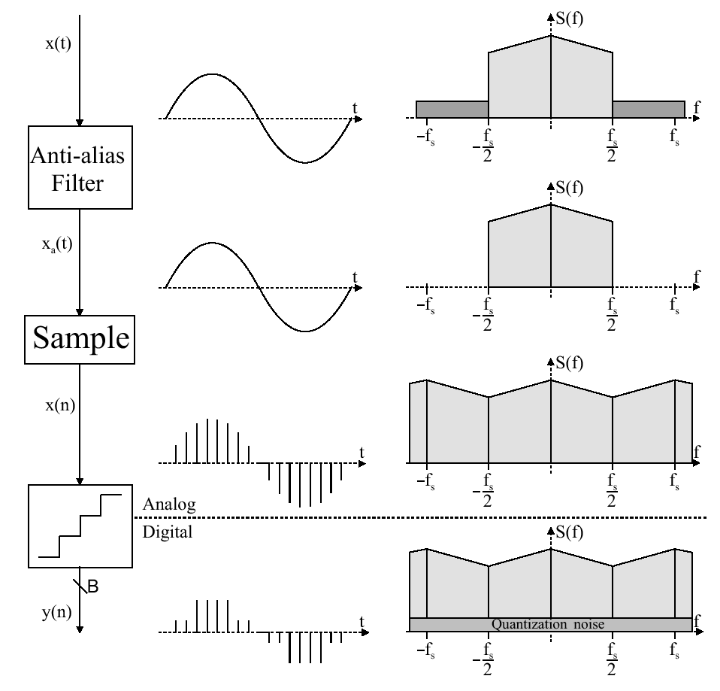
\includegraphics[width=0.65\linewidth]{conversion_chain.png}
    \caption{The conversion chain}
    \label{fig:conversion-chain-label}
\end{figure}

We first remove the alias, then sample it to go into discrete time. We then quantize sampled data which will inevitably introduce quantization error. Finally to reconstruct we will use a \textit{decimation filter}. In a Sigma-delta \gls{adc} we will use something called the \gls{osr} to improve this quantization noise.

\begin{equation}
    OSR = \frac{\text{sampling freq } f_s}{\text{Nyquist freq } 2 f_m}
\end{equation}

For the $n-$bit quantizer, it will introduce this infamous quantizer error that have a seesaw patern up until the overload area where it can no longer sample anything. This error is :

\begin{align}
    |V_{in}| &< x_{max} \quad |Q error| < \frac{\Delta}{2} & |V_{in}| &> x_{max} \quad \text{overload}
\end{align}

The quantization noise is a purely \textit{mathematical model}, it is not stochastic over time. It represents this transformation of a random input signal into a random output error due to quantization.\\

We can do the white noise approximation for fast varying signal where the error is evenly distributed between $[-\Delta/2;\Delta/2]$ with a pdf value of $1/\Delta$. We need no overload and need a change in input.

\begin{align}
    E(e_q) &= \frac{1}{\Delta I_R} \int_{-\frac{\Delta I_R}{2}}^{\frac{\Delta I_R}{2}} e de = 0 & \sigma_q^2&= \frac{1}{\Delta I_R} E((e_q-E(e_q))^2)\\
    & & &=\frac{1}{\Delta I_R} \int_{-\frac{\Delta I_R}{2}}^{\frac{\Delta I_R}{2}} e^2 de\\
    & & &= \frac{\Delta^2 I_R}{12}
\end{align}

The power is the \textit{variance} of the signal, which is equivalent to integrated noise. We only calculate the noise for a specific band.

\begin{align}
x_{\max} &= 2^B \frac{\Delta}{2} \frac{1}{k} \\ 
S &= y_{\text{rms}}^2 = (k x_{\text{rms}})^2 = k^2 \frac{x_{\max}^2}{2} \\ 
&= 2^{2B - 3} \Delta^2 \\ 
N &= \frac{\Delta^2}{12} \\ 
\Rightarrow SNR &= \frac{12}{8} 2^{2B} = \frac{3}{2} 2^{2B} = SNR_p = 1.76+6.02 B dB
\end{align}

By going over the sampling much more often we will spread this noise leading to better SNR performance.

\begin{align}
N_q &= \int_{-\frac{f_s}{2}}^{\frac{f_s}{2}} S_e^2(f) |H_e^2(f)| |H_d^2(f)| \, df = \int_{-f_b}^{f_b} h_e^2(f) \, df = \frac{\Delta^2}{12} \frac{2 f_b}{f_s} \\
&= \frac{\Delta^2}{12 \, OSR}
\end{align}

\begin{align}
SNR_p &= \frac{3}{2} 2^{2B} OSR & SNR_p &= 1.76 + 6.02 B  + 10 log(OSR) \text{ } dB
\end{align}

The main idea being delta sigma \gls{adc} is to take advantage of previous error and to integrate it (PI) to correct and go to better values. The \textit{delta} modulation comes from measuring the error and subtracting its output from the input. The storing (integrating in continuous time) is the principle of the \textit{delta-sigma} modulation.

\begin{figure}[H]
    \centering
    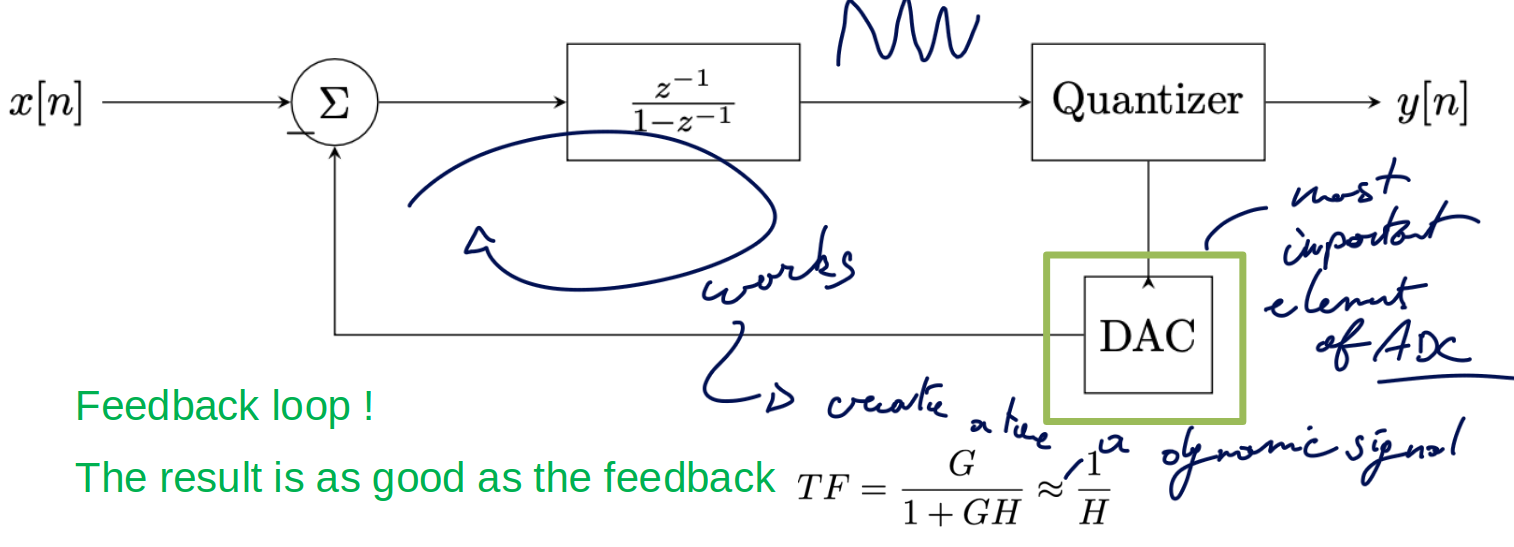
\includegraphics[width=0.75\linewidth]{delta_sigma.png}
    \caption{Delta sigma integration}
    \label{fig:delta-sigma-label}
\end{figure}

For the quantizer we can simply go for a comparator so $1$ or $-1$ and this is inherently linear. This will give us a noise and signal transfer function : 

\begin{align}
STF &= \frac{y}{x} = \frac{G}{1 + GH} & NTF &=  \frac{y}{e} = \frac{1}{1 + GH} \\ 
&= \frac{k \frac{1}{z-1}}{1 + k \frac{1}{z-1}} & &= \frac{1}{1 + k \frac{1}{z-1}}\\ 
&= \frac{k z^{-1}}{1 - z^{-1} + k z-1} & &= \frac{z-1}{z+(k-1)} \\ 
&= z^{-1} \quad \text{for } k = 1
\end{align}

We can clearly see the different transfer function which is a key aspect of delta sigma, it will do what we call \textit{noise shaping}. To get the continuous transfer function we can replace $z$ by $e^{j 2 \pi f/f_s}$. Again to find the SNR we have :

\begin{align}
    N_Q &= \int_{-f_b}^{f_b} \frac{\Delta^2}{12 f_s} NTF^2 df = \frac{\Delta^2}{4} \left(\frac{\pi}{3} \right)^2 \left( \frac{1}{OSR} \right)^3\\
    S &= \frac{\Delta 2^B}{2\sqrt{2}}\\
    SNR_{dB} &= 10 \cdot log(S) - 10 \cdot log(N_Q) = 6.02B-3.41+30\cdot log(OSR)  \label{eq:snr-noise}
\end{align}

One major approximation that this formula relies on is the $sin\left(\frac{2\pi}{OSR}\right) \approx \frac{2\pi}{OSR}$. So that's why we need high \gls{osr} values or we won't take advantage of this noise shaping.

\subsection{Second order Sigma Delta}

\begin{figure}[H]
    \centering
    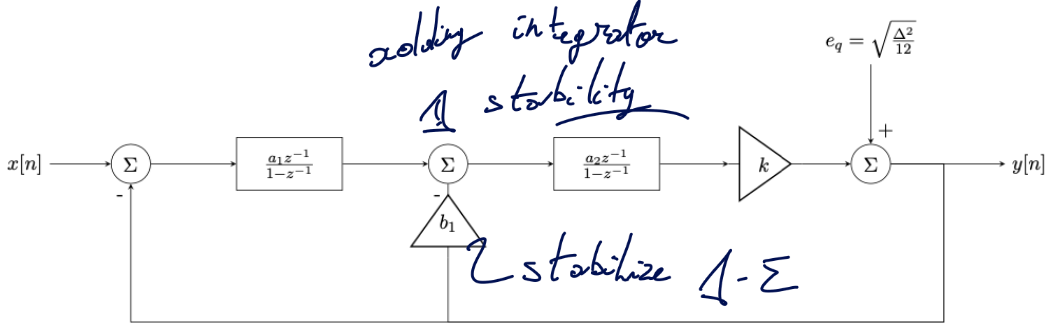
\includegraphics[width=0.75\linewidth]{second_order.png}
    \caption{Second order delta sigma}
    \label{fig:2-order-label}
\end{figure}

We can indeed have better noise shaping but we need to take into account potential instability of this loop. We need to pick the right $b_1$ for the job.

\begin{figure}[H]
    \centering
    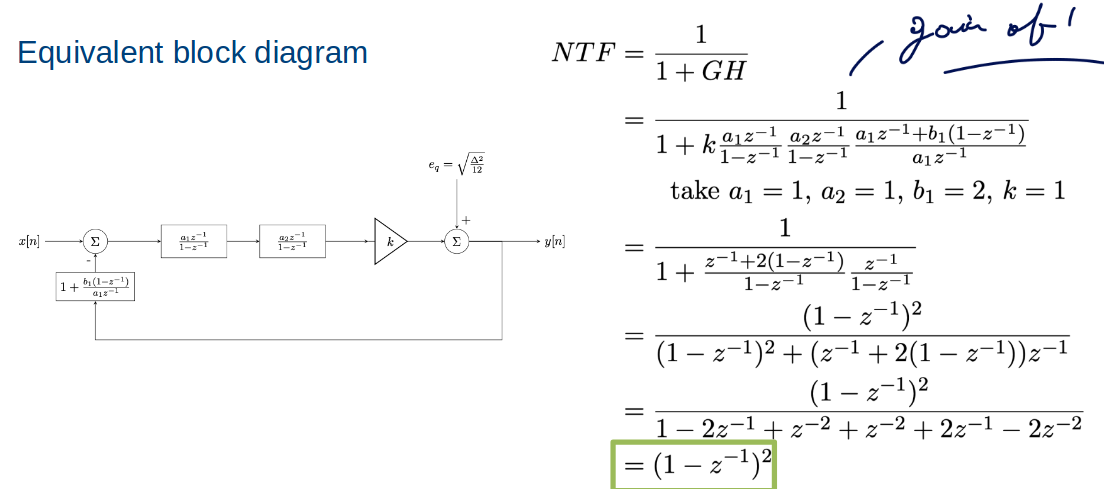
\includegraphics[width=0.75\linewidth]{equi_second_order.png}
    \caption{Equivalent second order}
    \label{fig:equi-2-order-label}
\end{figure}

Again, we can reapeat a similar process as in equation \ref{eq:snr-noise} and have :

\begin{align}
    SNR &= 6.02B-11.1 +50\cdot log(OSR)\\
    SNR_n &= 6.02B- 10\cdot log \left( \frac{2\pi^{2n}}{3(2n+1)} \right) +10(2n+1)\cdot log(OSR)
\end{align}

We can also have other issues that will limit our \gls{enob}, typically we can have third order distortion. But again, some paper will cheat and move the $f_{in}$ as close as the cut-off frequency so the third order distortion won't be seen.\\

The main action of a delta sigma, is converting a signal into a \gls{pwm} signal. But we could also face some saturation where the width of the signal doesn't reflect or mean any information. We need the amplitude to be lower as the feedback voltage to avoid \textit{overload}. Different order sigma delta have some different overload criteria, we will try to spread this swing to avoid overloading early stage integrator.

\subsection{Stability and Limit Cycle}

We know it is a feedback system so having the wrong coefficients will make an instable system. We can witness some \textit{limit cycle} as starting with some starting condition will evolve with the same trajectory. The instability can be seen as a loop that will go towards infinity and won't find stability. Usually, this will be limited by the supply range.

\subsubsection{Pattern noise}

There is a pattern in the ideal output at $f_s / 4$ and is called the limit cycle. Cause of this, the quantization is no longer white and we cannot longer do noise shaping. Dead zone in DC transfer function. We can use some matlab models to check for stability.

\textbf{page 51}



$$\nabla \times \left( \frac{1}{\mu} (\nabla \times \mathbf{A}) \right) = \mathbf{J} + \epsilon \frac{\partial}{\partial t} \left( -\nabla \Phi - \frac{\partial \mathbf{A}}{\partial t} \right)$$


\printglossary[type=\acronymtype]

\end{document}
